\documentclass[10pt, a4paper]{arbeitsblatt}

\ladeModule{theme,typo,icons,tabellen,boxen,aufgaben}
\aboptionen{
	name		= {J. Neugebauer},
	kuerzel		= {Ngb},
	titel		= {HTML-Tabellen},
	reihe		= {Webseiten erstellen mit HTML},
	fach		= {Informatik},
	lerngruppe	= {8Diff},
	nummer		= {II.5},
	lizenz		= {cc-by-nc-sa-4},
	version		= {2022-09-21},
}

\ladeFach[listings]{informatik}

\begin{document}
\ReiheTitel

Tabellen können auf Webseiten benutzt werden, um Informationen
strukturiert darzustellen.

\begin{figure}[ht]
	\begin{subfigure}[b]{.5\linewidth}
		\begin{lstlisting}[language=HTML]
<table border="1">
	<thead>
	<tr>
		<th>Monat</th>
		<th>Ersparnis</th>
	</tr>
	</thead>
	<tbody>
	<tr>
		<td>Januar</td>
		<td>100</td>
	</tr>
	<tr>
		<td>Februar</td>
		<td>80</td>
	</tr>
	</tbody>
	<tfoot>
	<tr>
		<td>Summe</td>
		<td>180</td>
	</tr>
	</tfoot>
</table>
		\end{lstlisting}
		\caption{Quelltext einer HTML-Tabelle}\label{lst:tabelle}
	\end{subfigure}%
	\begin{subfigure}[b]{.5\linewidth}\centering
		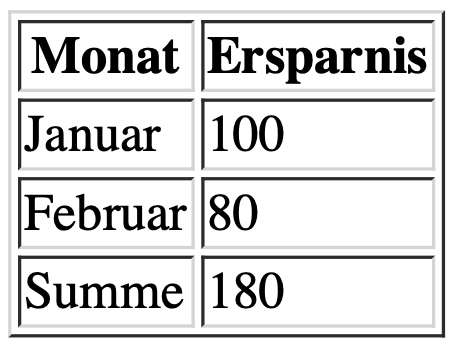
\includegraphics[width=3cm]{8Diff-AB.5-Abb_Tabelle.png}
		\caption{Darstellung im Webbrowser}\label{abb:tabelle-render}
	\end{subfigure}
	\caption{Eine HTML-Tabelle}\label{abb:tabelle}
\end{figure}

\begin{rahmen}\small
	In der Anfangszeit des World Wide Web wurden Tabellen darüber hinaus
	zum Design von Webseiten eingesetzt. Mit dem Aufkommen von Endgeräten
	mit unterschiedlichen Bildschirmgrößen wurde diese Praxis aber zugunsten
	des \emph{Responsiven Webdesigns} aufgegeben, da Webseiten mit einem
	tabellenbasierten Design keine Anpassungen zum Beispiel auf
	Smartphonegröße erlauben.
\end{rahmen}

\section*{Arbeitsaufträge}
\begin{aufgabe}[icon=\iconHeft]
	Analysiere den Quelltext einer HTML Tabelle oben links und vergleiche
	ihn mit der Darstellung auf der rechten Seite. Beschreibe, wie HTML
	Tabellen aufgebaut sind und versuche eine Erklärung für die einzelnen
	Tags zu finden.
\end{aufgabe}

\begin{aufgabe}[icon=\iconLaptop]
	Öffne die Webseite \url{https://link.ngb.schule/html-tabellen} und
	klicke oben auf \enquote{Run}. Modifiziere nun den Quelltext auf der
	linken Seite und erkunde, wie sich die Tabelle rechts verändert.
	Weitere Informationen findest du unter
	\url{https://www.html-seminar.de/attribute-bei-tabellen.htm}.
\end{aufgabe}

\begin{aufgabe}[icon=\iconLaptop]
	Erweitere deinen Steckbrief um eine HTML Tabelle, die die Informationen
	über dich strukturiert darstellt.
\end{aufgabe}

%\begin{aufgabe}
%	\begin{teilaufgaben}
%		\teilaufgabe\setzeIcon{\iconOhr} \textbf{(Ohne Computer)}
%		Analysiere den Quelltext einer HTML Tabelle oben links und vergleiche ihn mit der Darstellung auf der rechten Seite. Beschreibe, wie HTML Tabellen aufgebaut sind und versuche eine Erklärung für die einzelnen Tags zu finden.
%		\teilaufgabe \textbf{(Am Computer)}
%		Öffne die Webseite \url{https://link.ngb.schule/html-tabellen} und klicke oben auf \enquote{Run}. Modifiziere nun den Quelltext auf der linken Seite und erkunde, wie sich die Tabelle rechts verändert. Weitere Informationen findest du unter \url{https://www.html-seminar.de/attribute-bei-tabellen.htm}.
%		\teilaufgabe \textbf{(Am Computer)}
%		Erweitere deinen Steckbrief um eine HTML Tabelle, die die Informationen über dich strukturiert darstellt.
%	\end{teilaufgaben}
%\end{aufgabe}

\end{document}
